% =============================================================================
% Informe final — Billetera de Ahorro (Patrones de Diseño de APIs, MSOF-UPS)
% Compilar:  bash compilar.sh   (genera los capítulos desde Markdown y produce el PDF)
% =============================================================================
\documentclass[12pt,oneside]{report}
% =============================================================================
% Preámbulo del informe final — compilar con LuaLaTeX + Biber (ver compilar.sh)
% =============================================================================
\usepackage{fontspec}
\usepackage[spanish,es-noquoting,es-tabla]{babel}
\usepackage[a4paper,top=2.5cm,bottom=2.5cm,left=2.5cm,right=2.5cm,headheight=14pt]{geometry}
\usepackage{microtype}
\usepackage{xcolor}
\usepackage{graphicx}
\usepackage{float}
\usepackage{array,booktabs,longtable,tabularx,multirow,makecell,calc}
\usepackage{amssymb}
\usepackage{enumitem}
\usepackage{caption}
\usepackage{titlesec}
\usepackage{fancyhdr}
\usepackage{etoolbox}
\usepackage{listings}
\usepackage[most]{tcolorbox}
\usepackage{csquotes}
\usepackage[style=apa,backend=biber]{biblatex}
\usepackage[hidelinks,pdfusetitle]{hyperref}

\addbibresource{referencias.bib}

% --- Colores institucionales sobrios ------------------------------------------
\definecolor{azulups}{HTML}{003A70}
\definecolor{grisclaro}{HTML}{F2F4F7}
\definecolor{grismedio}{HTML}{6C757D}

% --- Títulos ---------------------------------------------------------------------
\titleformat{\chapter}[display]
  {\normalfont\bfseries\color{azulups}}
  {\large\MakeUppercase{\chaptertitlename}\ \thechapter}
  {6pt}{\Huge}
\titlespacing*{\chapter}{0pt}{-10pt}{24pt}
\titleformat{\section}{\normalfont\Large\bfseries\color{azulups}}{\thesection}{0.8em}{}
\titleformat{\subsection}{\normalfont\large\bfseries}{\thesubsection}{0.8em}{}
\setcounter{secnumdepth}{2}
\setcounter{tocdepth}{1}

% --- Encabezados -----------------------------------------------------------------
\pagestyle{fancy}
\fancyhf{}
\fancyhead[L]{\small\color{grismedio}Billetera de Ahorro}
\fancyhead[R]{\small\color{grismedio}\nouppercase{\rightmark}}
\renewcommand{\chaptermark}[1]{\markboth{#1}{#1}}
\renewcommand{\sectionmark}[1]{}
\fancyfoot[C]{\small\thepage}
\renewcommand{\headrulewidth}{0.3pt}
\fancypagestyle{plain}{\fancyhf{}\fancyfoot[C]{\small\thepage}\renewcommand{\headrulewidth}{0pt}}

% --- Párrafos y listas -----------------------------------------------------------------
\setlength{\parindent}{0pt}
\setlength{\parskip}{6pt plus 2pt}
\setlist{itemsep=2pt,topsep=4pt}
\renewcommand{\arraystretch}{1.25}

% --- Figuras y tablas (APA: título arriba, en cursiva) ------------------------------
\captionsetup{font=small,labelfont={bf,color=azulups},textfont=it,justification=raggedright,singlelinecheck=false}
\captionsetup[table]{position=top}
\setlength{\LTpre}{6pt}\setlength{\LTpost}{6pt}
\AtBeginEnvironment{longtable}{\small}

% --- Compatibilidad con el LaTeX que genera pandoc ----------------------------------
\newcounter{none} % tablas sin título (pandoc usa \LTcaptype{none})
\providecommand{\tightlist}{\setlength{\itemsep}{0pt}\setlength{\parskip}{0pt}}
\makeatletter
\newsavebox\pandoc@box
\newcommand*\pandocbounded[1]{%
  \sbox\pandoc@box{#1}%
  \Gscale@div\@tempa{\textheight}{\dimexpr\ht\pandoc@box+\dp\pandoc@box\relax}%
  \Gscale@div\@tempb{\linewidth}{\wd\pandoc@box}%
  \ifdim\@tempb\p@<\@tempa\p@\let\@tempa\@tempb\fi
  \ifdim\@tempa\p@<\p@\scalebox{\@tempa}{\usebox\pandoc@box}%
  \else\usebox{\pandoc@box}\fi}
\makeatother
\def\fps@figure{H}
\renewenvironment{quote}{\begin{tcolorbox}[colback=grisclaro,colframe=grisclaro,boxrule=0pt,left=8pt,right=8pt,top=4pt,bottom=4pt,sharp corners,breakable]}{\end{tcolorbox}}

% --- Código y evidencias de terminal ---------------------------------------------------
\lstset{
  basicstyle=\ttfamily\scriptsize,
  breaklines=true,
  breakatwhitespace=false,
  columns=fullflexible,
  keepspaces=true,
  frame=single,
  rulecolor=\color{grismedio!40},
  backgroundcolor=\color{grisclaro},
  inputencoding=utf8,
  extendedchars=true,
  literate={á}{{\'a}}1 {é}{{\'e}}1 {í}{{\'i}}1 {ó}{{\'o}}1 {ú}{{\'u}}1 {ñ}{{\~n}}1
           {Á}{{\'A}}1 {É}{{\'E}}1 {Í}{{\'I}}1 {Ó}{{\'O}}1 {Ú}{{\'U}}1 {Ñ}{{\~N}}1
           {→}{{$\rightarrow$}}1 {✓}{{$\checkmark$}}1 {×}{{$\times$}}1 {↳}{{$\hookrightarrow$}}1 {│}{{|}}1 {├}{{|}}1 {└}{{|}}1 {─}{{-}}1 {—}{{--}}1 {≈}{{$\approx$}}1 {·}{{$\cdot$}}1 {¿}{{?`}}1 {¡}{{!`}}1 {ü}{{\"u}}1 {…}{{...}}1 {•}{{$\bullet$}}1
}

% --- Recuadro para contenido pendiente ------------------------------------------------
\newtcolorbox{pendiente}{colback=yellow!8,colframe=orange!70!black,title=Pendiente,fonttitle=\bfseries,breakable}

% --- Datos del documento -------------------------------------------------------------
\newcommand{\titulo}{Billetera de Ahorro: plataforma de planes de ahorro programado dirigida por APIs}
\title{\titulo}
\author{Grupo del Trabajo Final — Patrones de Diseño de APIs}


\begin{document}

% Portada (formato institucional UPS, sin logotipo)
\begin{titlepage}
\centering
\color{azulups}
{\Large\bfseries UNIVERSIDAD POLITÉCNICA SALESIANA\par}
\vspace{4pt}
{\large Unidad de Posgrados\par}
{\large Maestría en Software\par}
\vspace{1.6cm}
{\normalcolor\large Asignatura: Patrones de Diseño de APIs\par}
\vspace{2.2cm}
{\normalcolor\large\scshape Informe final del proyecto\par}
\vspace{0.6cm}
\rule{0.85\linewidth}{0.8pt}\par
\vspace{0.4cm}
{\Huge\bfseries Billetera de Ahorro\par}
\vspace{0.3cm}
{\Large Plataforma de planes de ahorro programado dirigida por APIs\par}
\vspace{0.4cm}
\rule{0.85\linewidth}{0.8pt}\par
\vfill
\normalcolor
\begin{tabular}{@{}rl@{}}
\textbf{Docente:} & Ing. Patsy Malena Prieto, MSc. \\[4pt]
\textbf{Integrantes:} & \rule{7cm}{0.4pt} \\[4pt]
 & \rule{7cm}{0.4pt} \\[4pt]
 & \rule{7cm}{0.4pt} \\[4pt]
 & \rule{7cm}{0.4pt} \\[4pt]
 & \rule{7cm}{0.4pt} \\
\end{tabular}
\vfill
{\large Ecuador, octubre de 2026\par}
\end{titlepage}


\pagenumbering{roman}
\chapter*{Resumen}
\addcontentsline{toc}{chapter}{Resumen}

Este informe documenta el diseño y la construcción de la \emph{Billetera de Ahorro}, un producto bancario de planes de ahorro programado expuesto mediante APIs. El cliente fija una meta y una fecha objetivo, el sistema calcula la cuota mensual, la debita de forma automática de su cuenta y muestra el progreso; si el cliente bloquea el plan, obtiene una tasa preferencial.

El trabajo siguió las cuatro fases de la asignatura. En la Fase~1 justificamos el caso de negocio con un modelo de monetización indirecta basado en el spread y la permanencia de los depósitos. En la Fase~2 elegimos un estilo híbrido REST y orientado a eventos, desplegado como monolito modular detrás de un API Gateway, y justificamos sus patrones con la matriz ISO/IEC~25010. En la Fase~3 escribimos el contrato OpenAPI~3.1 antes que el código (contract-first). En la Fase~4 implementamos el backend en Node.js por capas, con JWT RS256, Circuit Breaker, Retry con jitter, Transactional Outbox e idempotencia; alcanzamos 97,9~\% de cobertura de líneas con 97 pruebas, desplegamos en AWS con un pipeline de CI/CD y medimos el sistema con k6: bajo carga sostenida de 200 usuarios el p95 fue de 336~ms con 0,001~\% de errores, y el punto de ruptura se ubicó en unas 220 peticiones por segundo, limitado por la base de datos. Finalmente integramos el frontend en Next.js con la API y lo publicamos en Azure App Service, desde donde recorrimos el flujo completo de punta a punta contra el backend en AWS.

\medskip
\textbf{Palabras clave:} API-First, OpenAPI, arquitectura orientada a eventos, patrones de resiliencia, JWT, pruebas de carga, CI/CD.

\tableofcontents
\listoffigures
\listoftables
\cleardoublepage
\pagenumbering{arabic}

\chapter{Introducción}\label{cap:introduccion}

\section{Contexto y problema}

El ahorro de las personas suele ser un residuo: se ahorra lo que sobra a fin de mes. Los productos tradicionales piden montos mínimos, plazos rígidos y trámites en agencia, y el cliente no sabe cuánto tendrá al final. Del lado del banco, el depósito a la vista es barato pero volátil, y la apertura de productos de ahorro en canales digitales se abandona sin que el banco sepa por qué.

La \emph{Billetera de Ahorro} responde a ambos problemas: automatiza el aporte, muestra desde el primer momento cuánto dinero tendrá el cliente y no exige monto mínimo. A cambio, el banco obtiene depósitos recurrentes y de mayor permanencia. El producto se construyó con un enfoque API-First: la capacidad de ahorro se expone como un contrato que hoy consume la banca web y mañana podrían consumir socios externos.

\section{Objetivos}

\textbf{Objetivo general.} Diseñar, implementar y desplegar una plataforma de planes de ahorro programado dirigida por APIs, aplicando los patrones de diseño y arquitectura vistos en la asignatura.

\textbf{Objetivos específicos.}
\begin{itemize}
  \item Justificar el caso de negocio, la cadena de valor y el modelo de monetización de la API (Fase~1).
  \item Seleccionar y justificar el estilo arquitectónico y los patrones de diseño (Fase~2).
  \item Especificar el modelo de datos y el contrato de la API con OpenAPI (Fase~3).
  \item Implementar los servicios con seguridad, pruebas, pruebas de carga y despliegue automatizado (Fase~4).
\end{itemize}

\section{Alcance}

El alcance aprobado por el equipo incluye la creación de varios planes con cuota fija mensual, la simulación pública, el débito automático con cinco intentos, los aportes y retiros, el bloqueo y desbloqueo del plan, la cancelación con devolución de fondos y la consulta del historial. El Core bancario y el sistema de notificaciones son sistemas existentes del banco: para el proyecto, el Core se simula sobre MongoDB Atlas y queda fuera del alcance del producto.

\section{Organización del repositorio y del documento}

Todo el trabajo está versionado en un repositorio de GitHub. La Tabla~\ref{tab:repositorio} resume su estructura.

\begin{table}[H]
\centering
\caption{Organización del repositorio}\label{tab:repositorio}
\begin{tabularx}{\linewidth}{@{}>{\ttfamily}l X@{}}
\toprule
\normalfont\textbf{Carpeta} & \textbf{Contenido} \\
\midrule
contracts/ & Contrato OpenAPI 3.1 (fuente de verdad de la API) \\
backend/ & Implementación en Node.js, pruebas, scripts de carga y despliegue \\
frontend/ & Aplicación web en Next.js \\
bdd/ & Modelo del Core bancario simulado (MongoDB) \\
docs/informes/ & Informes de cada fase en Markdown \\
docs/diagramas/ & Modelo C4 (Structurizr) y vista ArchiMate \\
docs/evidencias/ & Evidencias de pruebas, seguridad, despliegue y carga \\
docs/latex/ & Fuente de este informe \\
entregables/ & Documentos finales para la entrega \\
.github/workflows/ & Pipeline de CI/CD \\
\bottomrule
\end{tabularx}
\end{table}

Los capítulos~\ref{cap:fase1} a~\ref{cap:fase4} corresponden a las cuatro fases del proyecto. El capítulo~\ref{cap:frontend} describe la integración con el frontend y el capítulo~\ref{cap:conclusiones} presenta las conclusiones. Los anexos reúnen el detalle de los patrones de diseño y las evidencias.


\chapter{Fase 1: justificación de negocio}\label{cap:fase1}
\input{generados/fase1-negocio}
\section{Requerimientos del producto}
\input{generados/fase1-requerimientos}

\chapter{Fase 2: arquitectura y patrones}\label{cap:fase2}
\input{generados/fase2-arquitectura}

\chapter{Fase 3: modelo de datos y contrato de la API}\label{cap:fase3}

\section{Enfoque contract-first}

Escribimos el contrato antes que el código. El archivo \texttt{contracts/openapi.yaml} (OpenAPI~3.1) es la única fuente de verdad entre el frontend y el backend: los DTOs de validación del backend, los tipos del frontend y las pruebas siguen su forma. El contrato se valida con Redocly en cada ejecución del pipeline y se publica con Swagger UI junto con la API, en \texttt{http://3.151.57.252/docs/} (Figura~\ref{fig:swagger}).

\begin{figure}[H]
\centering
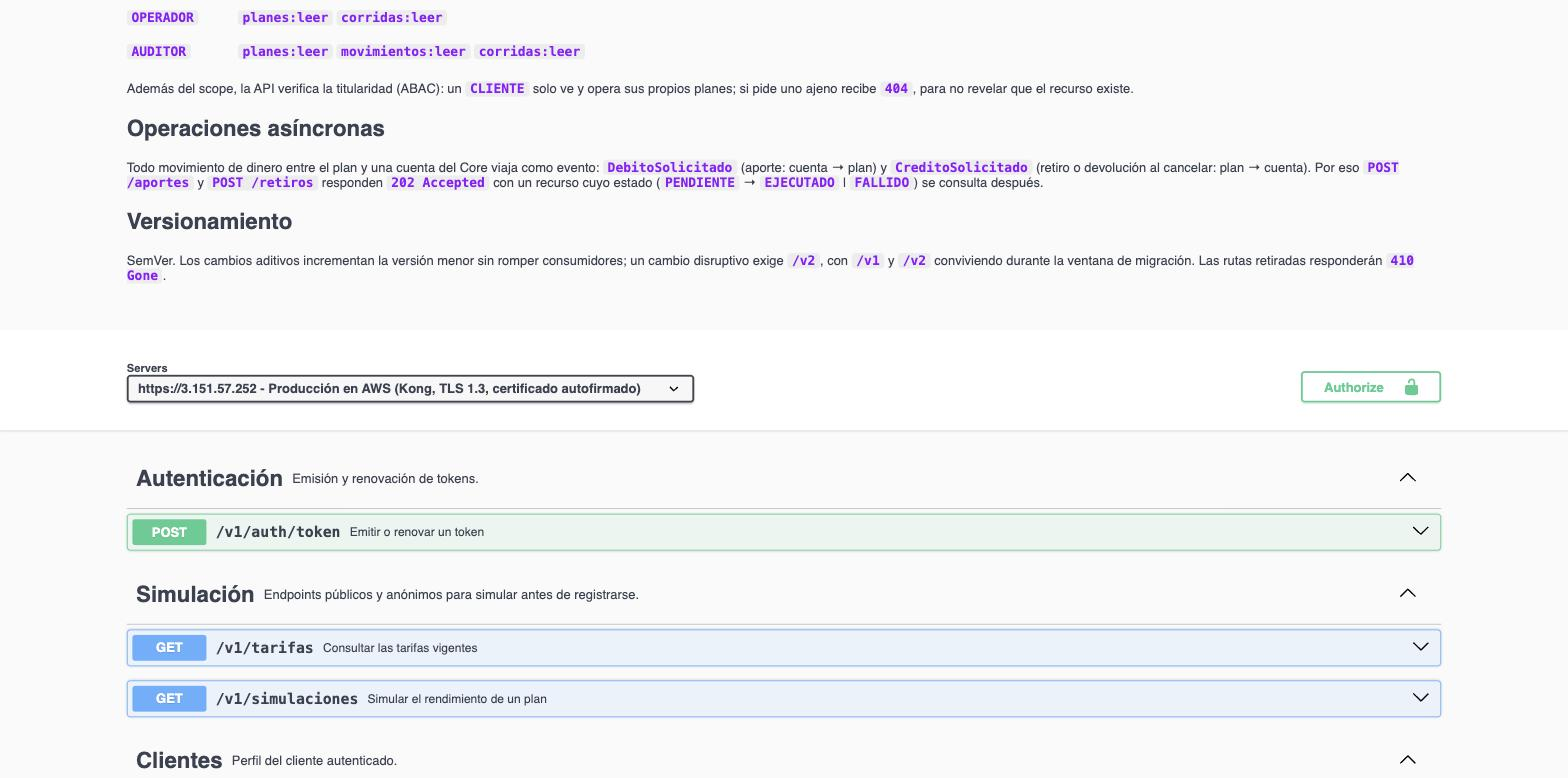
\includegraphics[width=\linewidth]{../evidencias/fase-3-contrato/swagger-ui-endpoints.jpg}
\caption{Contrato publicado con Swagger UI en el entorno de AWS}\label{fig:swagger}
\end{figure}

\section{Convenciones del contrato}

\begin{table}[H]
\centering
\caption{Convenciones de diseño del contrato}\label{tab:convenciones}
\begin{tabularx}{\linewidth}{@{}>{\raggedright}p{3.2cm} X@{}}
\toprule
\textbf{Aspecto} & \textbf{Decisión} \\
\midrule
Rutas & Sustantivos en plural y versión mayor en la ruta (\texttt{/v1}). Las acciones que no son CRUD son sub-recursos (\texttt{/bloqueo}, \texttt{/desbloqueo}, \texttt{/cancelacion}, \texttt{/aportes}, \texttt{/retiros}). No hay \texttt{DELETE}: el historial financiero no se borra. \\
Montos & Enteros en centavos (\texttt{*Centavos}) junto con el código ISO~4217; nunca decimales para dinero. \\
Fechas & ISO~8601: \texttt{date} para fechas de calendario y \texttt{date-time} en UTC para instantes. \\
Errores & \texttt{application/problem+json} (RFC~9457) con un \texttt{codigo} estable para el consumidor. \\
Paginación & Offset (\texttt{pagina}, \texttt{limite}) en planes, cuotas y corridas; cursor opaco (\texttt{cursor}, \texttt{limite}) en movimientos, que crecen sin límite. \\
Operaciones asíncronas & Aportes y retiros responden \texttt{202 Accepted} con un recurso cuyo estado (\texttt{PENDIENTE}, \texttt{EJECUTADO}, \texttt{FALLIDO}) se consulta en \texttt{Location}. \\
Concurrencia & \texttt{Idempotency-Key} en las operaciones que mueven dinero; \texttt{ETag}/\texttt{If-Match} al modificar un plan (412 si cambió). \\
Seguridad & Esquema \texttt{bearerAuth} (JWT); cada operación declara los scopes que exige. \\
Versionamiento & SemVer: los cambios aditivos suben la versión menor; un cambio disruptivo exige \texttt{/v2}. \\
\bottomrule
\end{tabularx}
\end{table}

\section{Modelo de datos orientado a la API}

El modelo que expone la API no copia las tablas de la base de datos: representa lo que el consumidor necesita. Por ejemplo, el saldo del plan no se almacena, se calcula desde el ledger; el progreso es un campo calculado; y la cuenta de débito viaja enmascarada. La Tabla~\ref{tab:recursos} resume los recursos.

\begin{table}[H]
\centering
\caption{Recursos del modelo de la API}\label{tab:recursos}
\begin{tabularx}{\linewidth}{@{}>{\ttfamily\raggedright}p{3.1cm} X@{}}
\toprule
\normalfont\textbf{Recurso} & \textbf{Contenido y reglas} \\
\midrule
PlanAhorro & Meta y fecha objetivo, cuota calculada, plazo y prórrogas, día de débito, cuenta, bloqueo, tasas (TNA base, bono, total y TEA), saldo y saldo disponible derivados del ledger, intereses devengados, progreso, estado (\texttt{ACTIVO}, \texttt{COMPLETADO}, \texttt{CANCELADO}). \\
Simulacion & Cuota mensual, total aportado, intereses proyectados, monto final y proyección mes a mes. Pública y cacheable. \\
TablaTarifas & Tramos de tasa por plazo y bono por bloqueo. \\
Cuota & Calendario de débitos con estado (\texttt{PROGRAMADA}, \texttt{PENDIENTE}, \texttt{EJECUTADA}, \texttt{CANCELADA}) e intentos (máximo 5). \\
Aporte / Retiro & Movimiento de dinero asíncrono con la cuenta del Core, su estado, el motivo de fallo y el \texttt{correlationId}. \\
Movimiento & Asiento del ledger de solo inserción, con el saldo resultante. \\
CuentaDebito & Cuenta del cliente en el Core, enmascarada, con su saldo disponible. \\
CorridaCobro & Resultado de cada corte diario del Batch (para operación y auditoría). \\
Cliente / Token & Perfil del cliente y par de tokens JWT. \\
Problema & Detalle de error RFC~9457 con \texttt{codigo} y errores por campo. \\
\bottomrule
\end{tabularx}
\end{table}

La persistencia, en cambio, está normalizada en PostgreSQL: \texttt{planes}, \texttt{cuotas}, \texttt{operaciones\_core}, el ledger \texttt{movimientos} (protegido por un trigger que rechaza UPDATE y DELETE), \texttt{outbox}, \texttt{eventos\_procesados}, \texttt{idempotencia} y \texttt{corridas\_cobro}. La vista \texttt{vw\_planes} deriva el saldo, los intereses y el monto reservado por retiros pendientes, y el procedimiento \texttt{sp\_procesar\_debitos\_ahorro\_programado} solo selecciona las cuotas a cobrar.

\section{Operaciones del contrato}

La Tabla~\ref{tab:endpoints} lista las 20 operaciones del contrato con el scope que exige cada una y los códigos de estado que documenta. Se genera automáticamente desde el archivo OpenAPI, así que no puede quedar desactualizada respecto del contrato.

\input{generados/fase3-endpoints}

\section{Ajuste del contrato al frontend}

Al revisar el frontend que construyó el equipo, ajustamos el contrato y el alcance: el login pasó a ser por email; la creación del plan usa una fecha objetivo y el sistema calcula la cuota; se agregaron el retiro parcial (RF-04.3) y el desbloqueo con pérdida de los intereses devengados (RF-01.7), con el evento \texttt{CreditoSolicitado} simétrico al débito; y se incorporaron el perfil del cliente, el saldo de las cuentas y un resumen de totales en el listado de planes. Estos cambios se reflejaron en los requerimientos, en la Fase~2 y en el diagrama C4.

\section{Validación}

El contrato se valida con Redocly sin errores (Anexo~\ref{anx:evidencias}). Las dos advertencias restantes corresponden a la URL de servidor local (\texttt{localhost}), que se mantiene a propósito para el entorno de desarrollo.


\chapter{Fase 4: desarrollo, seguridad y despliegue}\label{cap:fase4}
\input{generados/fase4-desarrollo}

\chapter{Integración con el frontend y pruebas de extremo a extremo}\label{cap:frontend}

El frontend (Next.js~16, React~19 y Zustand) se diseñó desde el principio con la forma del contrato: montos en centavos, los mismos estados del plan y los mismos códigos de error. En esta etapa se reemplazaron sus datos de prueba por llamadas a la API desplegada en AWS y se publicó en Azure App Service. Así la solución quedó repartida en dos nubes: la API y su Gateway en AWS, y la aplicación web en Azure.

\section{Arquitectura de la integración}

\begin{table}[H]
\centering
\caption{Piezas del frontend que consumen la API}\label{tab:front-piezas}
\begin{tabularx}{\linewidth}{@{}>{\ttfamily\raggedright}p{3.6cm} X@{}}
\toprule
\textbf{\normalfont Pieza} & \textbf{Responsabilidad} \\
\midrule
lib/api.ts & Cliente HTTP. Agrega el access token, genera la \texttt{Idempotency-Key} en las operaciones que crean recursos o mueven dinero, renueva el token una vez ante un 401 y convierte las respuestas \texttt{application/problem+json} en errores con el \texttt{codigo} del contrato. \\
lib/auth-store.ts & Sesión: \texttt{POST /v1/auth/token} con contraseña o refresh token y \texttt{GET /v1/clientes/me}. Si varias peticiones reciben 401 a la vez, comparten una sola renovación. \\
lib/store.ts & Estado de la aplicación conectado a la API: planes con su resumen, cuentas, tarifas, movimientos por cursor y las acciones sobre el plan. \\
next.config.ts & Proxy del mismo origen: \texttt{/api/*} se reenvía al API Gateway. \\
\bottomrule
\end{tabularx}
\end{table}

\paragraph{Proxy del mismo origen.} Azure sirve el frontend solo por HTTPS, y el navegador bloquea las llamadas de una página HTTPS a un servidor HTTP (contenido mixto). Por eso el navegador no llama directamente al Gateway: llama a \texttt{/api/...} en el mismo dominio, y el servidor de Next.js reenvía la petición a AWS. Con este diseño tampoco hace falta CORS. Al exponer el Gateway directamente al navegador durante el desarrollo apareció un problema: el plugin \texttt{jwt} de Kong rechazaba la verificación previa de CORS (\texttt{OPTIONS}), que no lleva token. Se corrigió con \texttt{run\_\allowbreak{}on\_\allowbreak{}preflight: false}, para que esas peticiones las atienda el plugin \texttt{cors}.

\begin{table}[H]
\centering
\caption{Operaciones del contrato que usa cada pantalla}\label{tab:front-pantallas}
\begin{tabularx}{\linewidth}{@{}>{\raggedright}p{3.2cm} X@{}}
\toprule
\textbf{Pantalla} & \textbf{Operaciones} \\
\midrule
Ingreso & \texttt{POST /v1/auth/token}, \texttt{GET /v1/clientes/me} \\
Dashboard & \texttt{GET /v1/planes-ahorro} (con \texttt{resumen}), \texttt{GET /v1/cuentas-debito} \\
Nuevo plan & \texttt{GET /v1/simulaciones}, \texttt{GET /v1/cuentas-debito}, \texttt{POST /v1/planes-ahorro} \\
Detalle del plan & \texttt{GET /v1/planes-ahorro/\{id\}}, \texttt{GET /\{id\}/movimientos} (cursor), \texttt{GET /v1/tarifas}, \texttt{POST /\{id\}/bloqueo}, \texttt{/desbloqueo} y \texttt{/cancelacion} \\
Aportar y retirar & \texttt{POST /\{id\}/aportes} y \texttt{/retiros} (202), \texttt{GET} de la URL indicada en \texttt{Location} \\
\bottomrule
\end{tabularx}
\end{table}

\section{Operaciones asíncronas en la interfaz}

Un aporte o un retiro responde \texttt{202 Accepted} con la cabecera \texttt{Location} del recurso creado. La interfaz muestra ``Esperando la confirmación del banco'' y consulta esa URL cada 800~ms, durante 15~s como máximo, hasta que el estado deja de ser \texttt{PENDIENTE}:

\begin{itemize}
  \item \texttt{EJECUTADO}: se recargan el plan, el historial, el resumen y los saldos de las cuentas.
  \item \texttt{FALLIDO}: se muestra el motivo (\texttt{FONDOS\_\allowbreak{}INSUFICIENTES}, \texttt{CUENTA\_\allowbreak{}BLOQUEADA} o \texttt{CORE\_\allowbreak{}NO\_\allowbreak{}DISPONIBLE}) en lenguaje del usuario.
  \item Sin respuesta dentro de los 15~s: se informa que el banco sigue procesando la operación y que se reflejará en unos segundos.
\end{itemize}

La simulación del plan nuevo se pide al servidor (\texttt{GET /v1/simulaciones}) cuando el usuario deja de escribir durante 400~ms. Así la cuota y las tasas salen de la misma estrategia de cálculo que usa el backend, y no se consume el límite de peticiones en cada tecla.

\section{Despliegue en Azure}

\begin{table}[H]
\centering
\caption{Recursos del frontend en Azure}\label{tab:azure}
\begin{tabularx}{\linewidth}{@{}>{\raggedright}p{3.6cm} X@{}}
\toprule
\textbf{Recurso} & \textbf{Configuración} \\
\midrule
Suscripción & Azure for Students. Su política solo permite cinco regiones; se eligió \texttt{canadacentral}, la más cercana a la API en \texttt{us-east-2}. \\
Plan de App Service & \texttt{billetera-ahorro-plan}, Linux, nivel F1 (gratuito). \\
Aplicación web & \texttt{billetera-ahorro-front}: Node~24 LTS, servidor \texttt{standalone} de Next.js (\texttt{node server.js}), solo HTTPS, TLS mínimo 1.3 y FTP deshabilitado. \\
Identidad para CI/CD & Identidad administrada \texttt{billetera-ahorro-github} con credencial federada (OIDC) para la rama \texttt{main} del repositorio (el \emph{subject} incluye los identificadores numéricos del dueño y del repositorio, formato que GitHub envía para este repositorio) y el rol \emph{Website Contributor} limitado al grupo de recursos. No hay contraseñas guardadas en GitHub. \\
\bottomrule
\end{tabularx}
\end{table}

Dos workflows de GitHub Actions completan el despliegue:

\begin{itemize}
  \item \textbf{Frontend CI/CD} (\texttt{frontend-ci-cd.yml}): lint, verificación de tipos y compilación; empaqueta el servidor \texttt{standalone}, lo despliega en App Service y verifica que la aplicación responda. Si la aplicación está apagada, omite el despliegue en lugar de fallar.
  \item \textbf{Azure - encender o apagar} (\texttt{azure-frontend.yml}): enciende, apaga o consulta la aplicación y, opcionalmente, la instancia EC2 del backend. Así la demostración se levanta con un solo clic y fuera de ella no se consumen recursos.
\end{itemize}

La primera ejecución del pipeline del frontend reveló dos problemas que no aparecían en el entorno local:
\begin{itemize}
  \item La verificación de tipos fallaba porque los tipos globales de Next.js (\texttt{.next/types}) no existen en un checkout limpio. Se agregó \texttt{next typegen} antes de \texttt{tsc}.
  \item El inicio de sesión en Azure fallaba (\texttt{AADSTS700213}), porque GitHub envía para este repositorio un \emph{subject} OIDC con los identificadores numéricos del dueño y del repositorio. Se ajustó la credencial federada.
\end{itemize}
Con ambas correcciones, el pipeline compiló, desplegó en App Service y verificó el sitio. Después, el workflow de encendido y apagado detuvo la aplicación web y la instancia EC2 en una sola ejecución (Anexo~\ref{anx:evidencias}).

Las verificaciones del Anexo~\ref{anx:evidencias} confirman lo siguiente:
\begin{itemize}
  \item Las páginas responden 200 y el proxy entrega \texttt{/v1/tarifas} desde AWS.
  \item Una operación privada sin token responde 401.
  \item HTTP redirige a HTTPS.
  \item TLS~1.2 se rechaza y TLS~1.3 se acepta.
  \item Con la aplicación detenida, el sitio responde 403, y al encenderla vuelve a responder 200.
\end{itemize}

Una limitación conocida: el rate limiting de Kong cuenta por dirección IP, y detrás del proxy todas las peticiones llegan desde la IP del servidor de Azure. El límite del login (30 por minuto) se comparte entre todos los usuarios, lo que es suficiente para la demostración. En producción habría que propagar la IP del cliente (\texttt{X-Forwarded-For}) o limitar por consumidor.

\section{Pruebas de extremo a extremo}

Se recorrió el flujo completo en el navegador contra el sitio publicado en Azure, que a su vez usa la API en AWS. El usuario fue el cliente de prueba Pablo Jara, con las cuentas del Core simulado en MongoDB Atlas. En la Tabla~\ref{tab:e2e} se resume el resultado de cada paso.

\begin{table}[H]
\centering
\caption{Resultado de las pruebas de extremo a extremo}\label{tab:e2e}
\begin{tabularx}{\linewidth}{@{}>{\raggedright}p{3.6cm} X@{}}
\toprule
\textbf{Paso} & \textbf{Resultado} \\
\midrule
Ingreso & Sesión iniciada; el dashboard muestra los saldos reales de las tres cuentas del Core (Figura~\ref{fig:e2e-dashboard}). \\
Simulación y creación & Meta de \$1.200 al 1 de octubre de 2027: cuota de \$97,96 durante 12 meses a 4,50~\% TNA (4,59~\% TEA). Plan creado con 201 (Figura~\ref{fig:e2e-simulacion}). \\
Aportes & \$150 y \$50 desde la cuenta \texttt{pablo.viajes}: estado \texttt{PENDIENTE} y luego \texttt{EJECUTADO}. El saldo del plan pasa a \$200, y tras el primer aporte el de la cuenta baja de \$2.340,50 a \$2.190,50 (Figuras~\ref{fig:e2e-pendiente} y~\ref{fig:e2e-aporte}). \\
Retiro & \$30 hacia la misma cuenta: el saldo del plan queda en \$170. \\
Bloqueo y desbloqueo & Con el bloqueo, la tasa sube a 5,60~\% (4,50 de base más 1,10 de bono del tramo de 12 a 23 meses) y la interfaz indica que el plan no admite retiros. Al desbloquear, la interfaz advierte la pérdida de la tasa preferencial y la tasa vuelve a 4,50~\% (Figuras~\ref{fig:e2e-bloqueo} y~\ref{fig:e2e-desbloqueo}). \\
Historial & Los tres movimientos aparecen con su saldo resultante (Figura~\ref{fig:e2e-historial}). \\
Cancelación & El plan pasa a \texttt{CANCELADO} y su débito automático queda finalizado (Figura~\ref{fig:e2e-cancelado}). \\
\bottomrule
\end{tabularx}
\end{table}

\paragraph{Hallazgo: saldo desactualizado por la caché HTTP.} En la primera prueba, el aporte se registró en el backend, pero la pantalla seguía mostrando un saldo de \$0. La causa fue la siguiente:
\begin{itemize}
  \item El \texttt{ETag} del plan es su número de versión, que sirve para el control de concurrencia con \texttt{If-Match}. Un aporte cambia el saldo pero no la versión.
  \item El navegador revalidaba la respuesta con \texttt{If-None-Match}, la API contestaba \texttt{304 Not Modified} y el navegador reutilizaba el cuerpo anterior.
\end{itemize}
Se corrigió en las dos capas. Las respuestas privadas de la API ahora llevan \texttt{Cache-Control: no-store}, que además es la práctica recomendada para datos financieros, y una prueba unitaria lo verifica. El cliente HTTP del frontend tampoco usa la caché del navegador. Después de desplegar ambos cambios, el segundo aporte actualizó el saldo en pantalla sin recargar la página.

\begin{figure}[H]
\centering
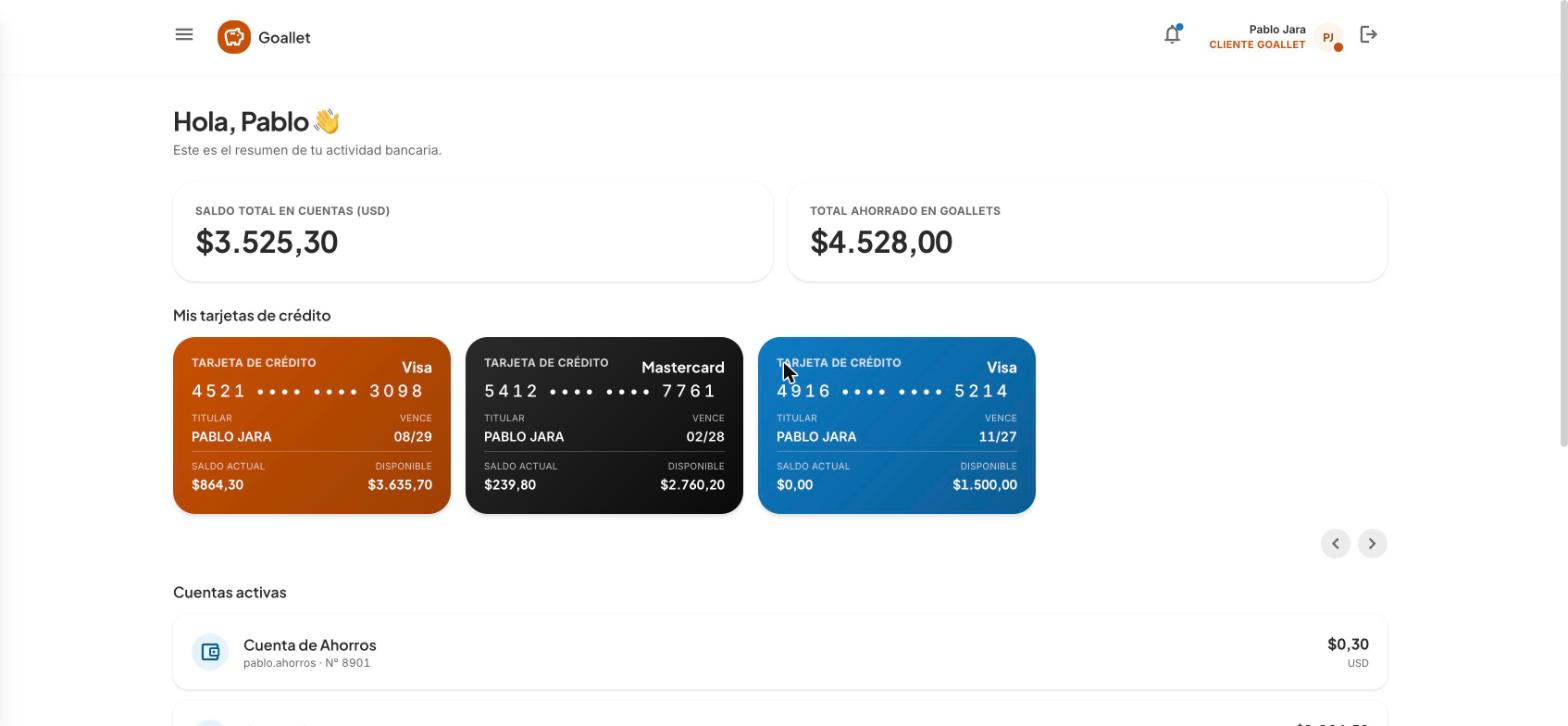
\includegraphics[width=0.9\linewidth]{../evidencias/fase-4-despliegue-frontend/02-dashboard.jpg}
\caption{Dashboard con los saldos de las cuentas obtenidos del Core}\label{fig:e2e-dashboard}
\end{figure}

\begin{figure}[H]
\centering
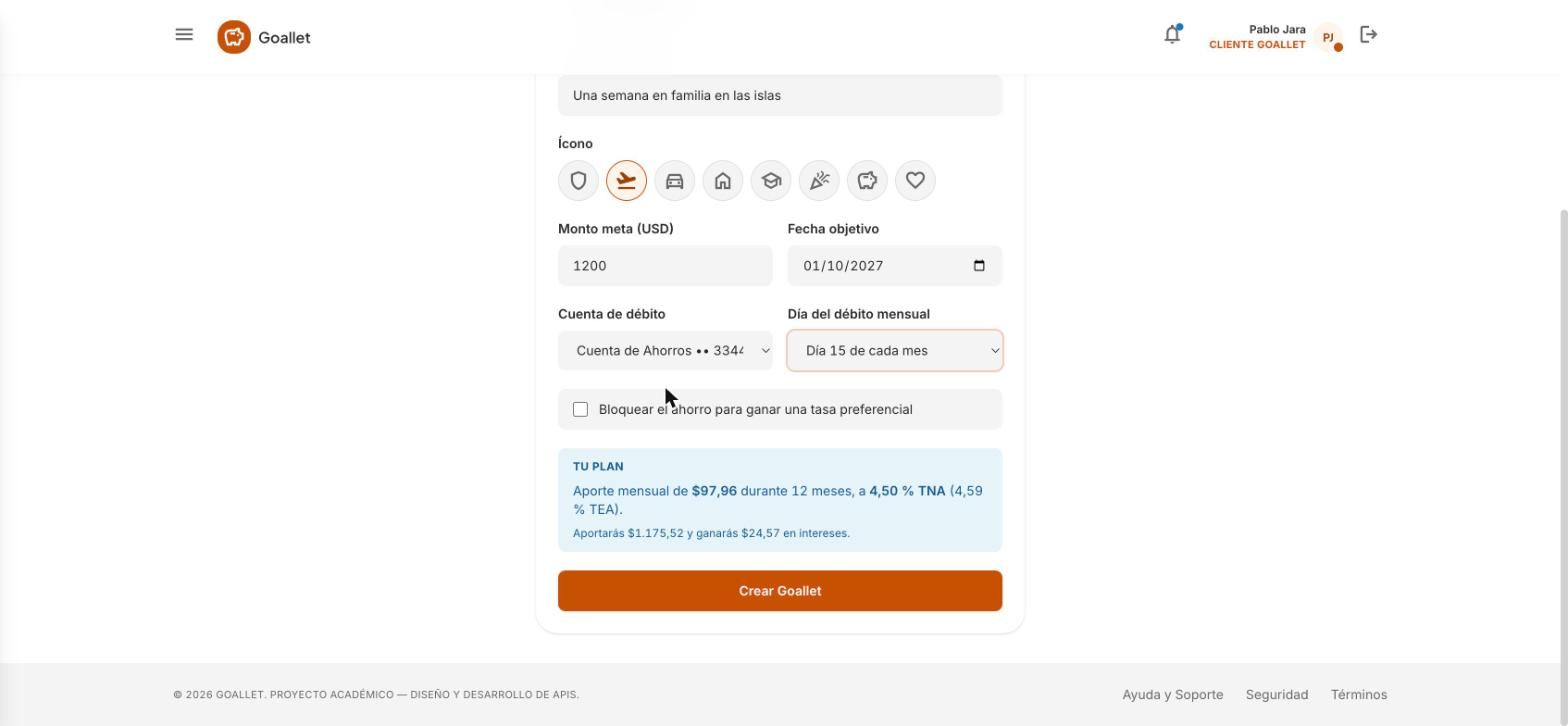
\includegraphics[width=0.9\linewidth]{../evidencias/fase-4-despliegue-frontend/04-nuevo-plan-simulacion.jpg}
\caption{Nuevo plan con la simulación calculada por la API}\label{fig:e2e-simulacion}
\end{figure}

\begin{figure}[H]
\centering
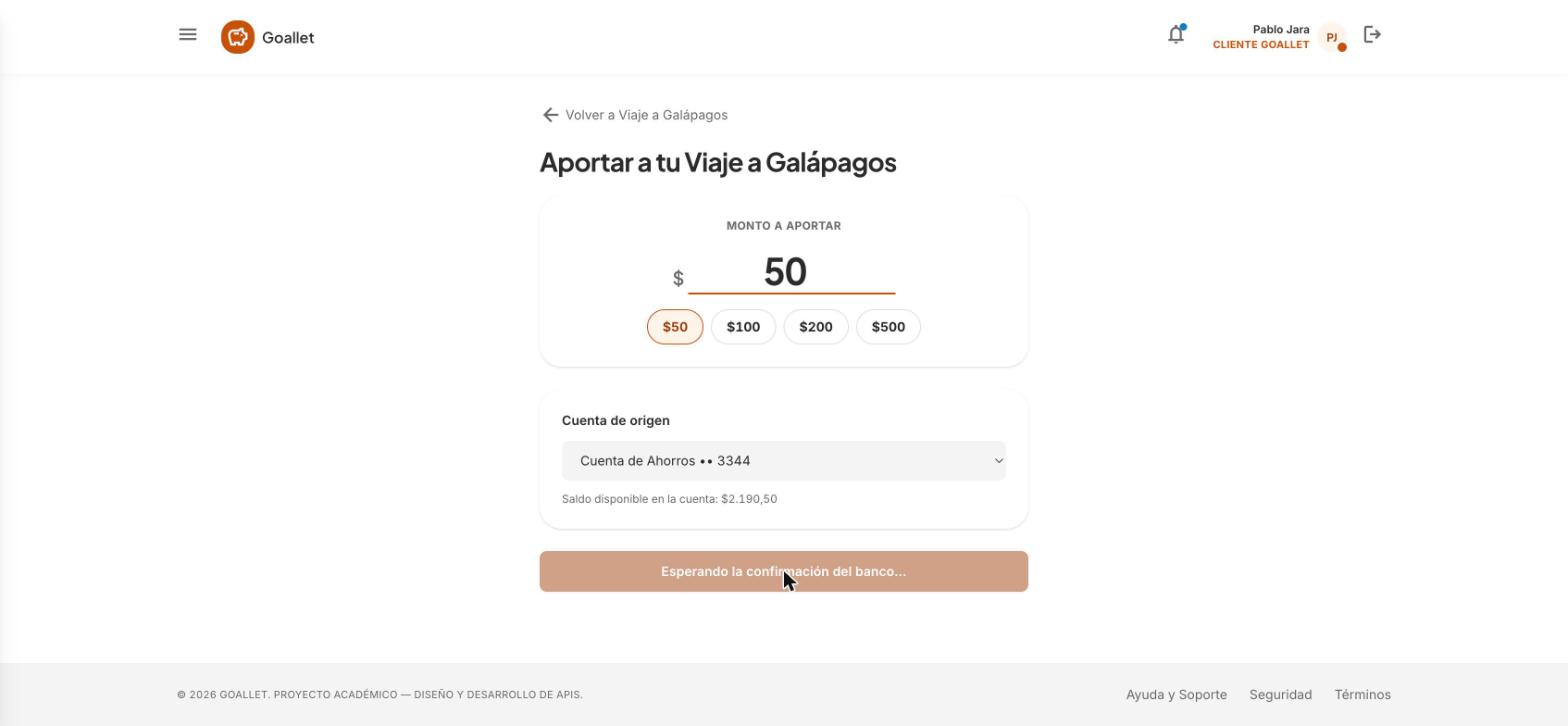
\includegraphics[width=0.9\linewidth]{../evidencias/fase-4-despliegue-frontend/07-aporte-esperando-core.jpg}
\caption{Aporte aceptado (202) a la espera de la confirmación del Core}\label{fig:e2e-pendiente}
\end{figure}

\begin{figure}[H]
\centering
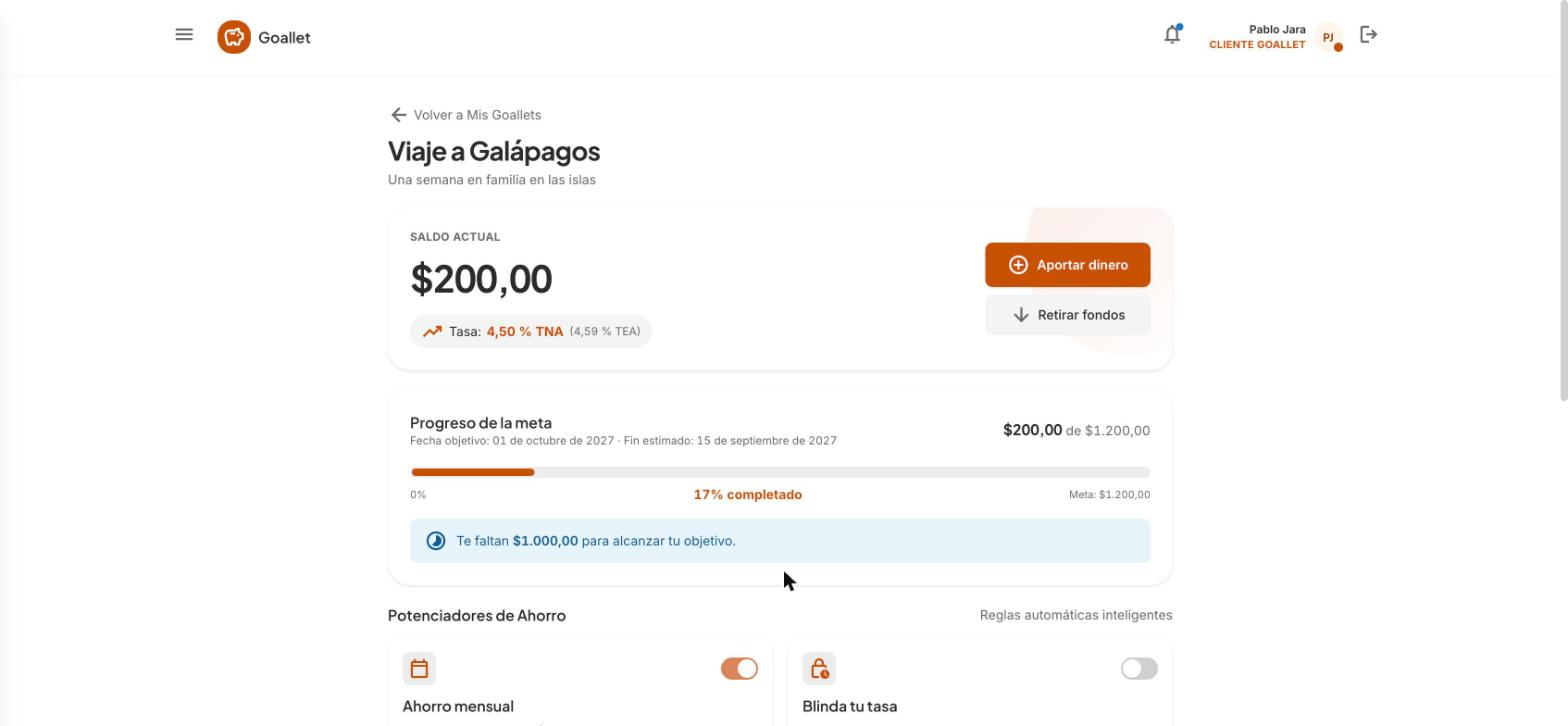
\includegraphics[width=0.9\linewidth]{../evidencias/fase-4-despliegue-frontend/08-aporte-confirmado.jpg}
\caption{Saldo actualizado después de la confirmación del aporte}\label{fig:e2e-aporte}
\end{figure}

\begin{figure}[H]
\centering
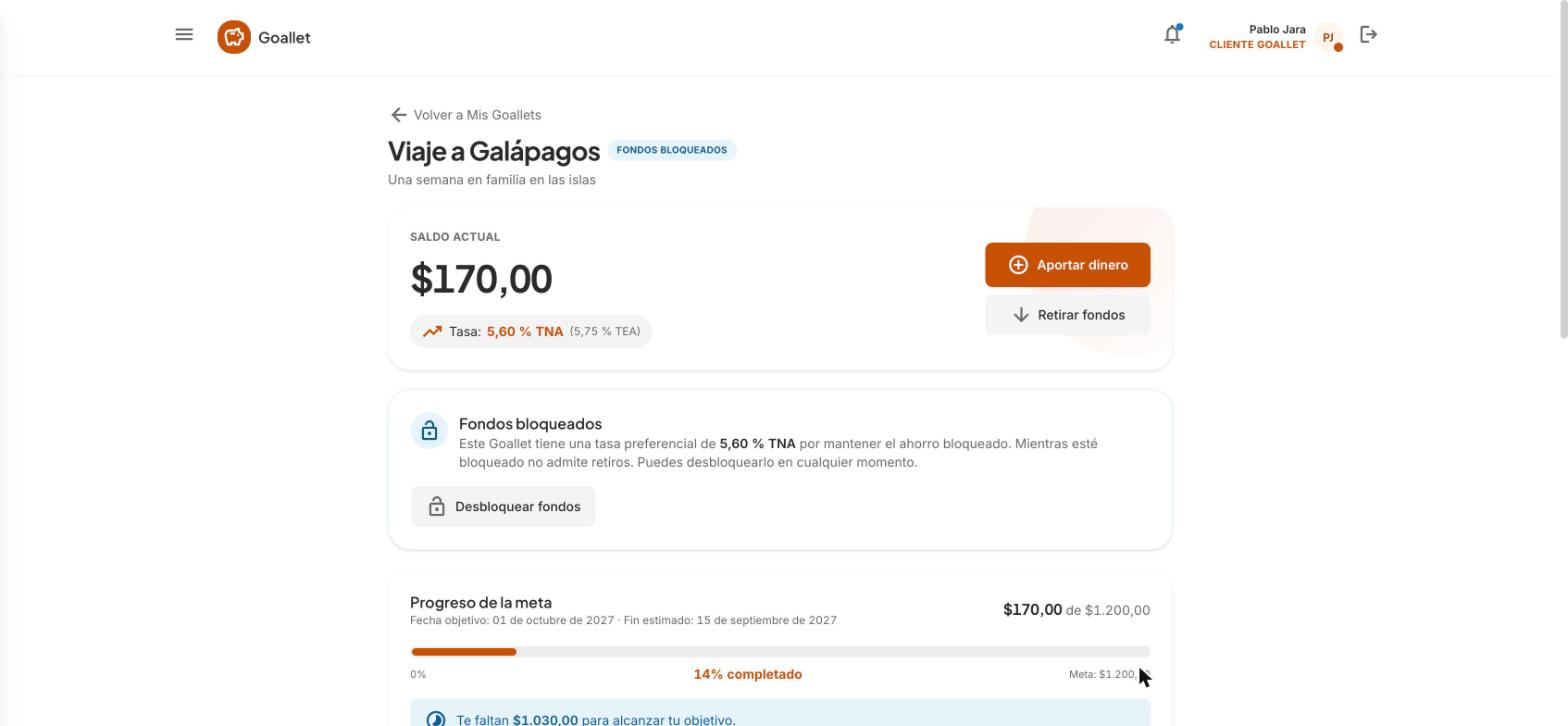
\includegraphics[width=0.9\linewidth]{../evidencias/fase-4-despliegue-frontend/11-plan-bloqueado.jpg}
\caption{Plan bloqueado con la tasa preferencial}\label{fig:e2e-bloqueo}
\end{figure}

\begin{figure}[H]
\centering
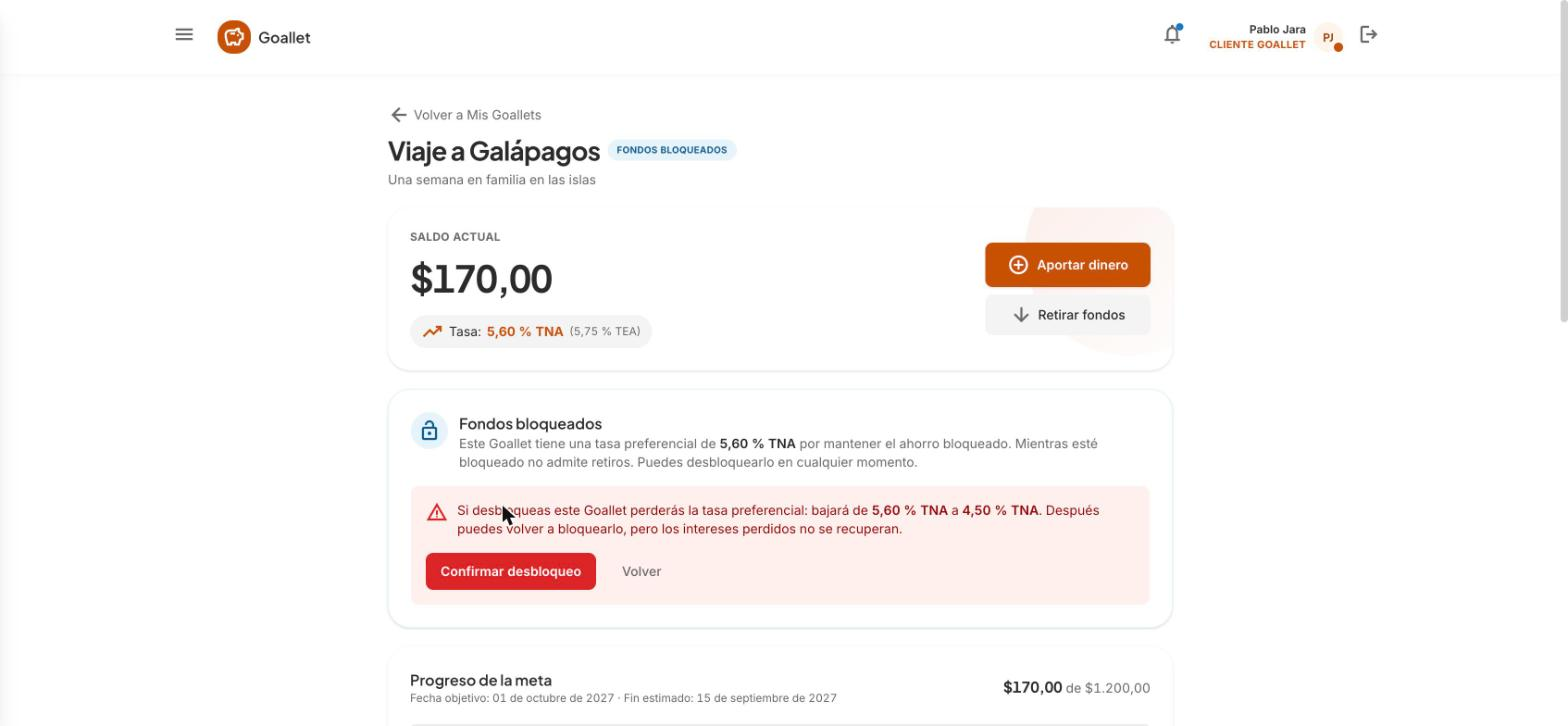
\includegraphics[width=0.9\linewidth]{../evidencias/fase-4-despliegue-frontend/12-desbloqueo-confirmacion.jpg}
\caption{Advertencia antes de desbloquear el plan}\label{fig:e2e-desbloqueo}
\end{figure}

\begin{figure}[H]
\centering
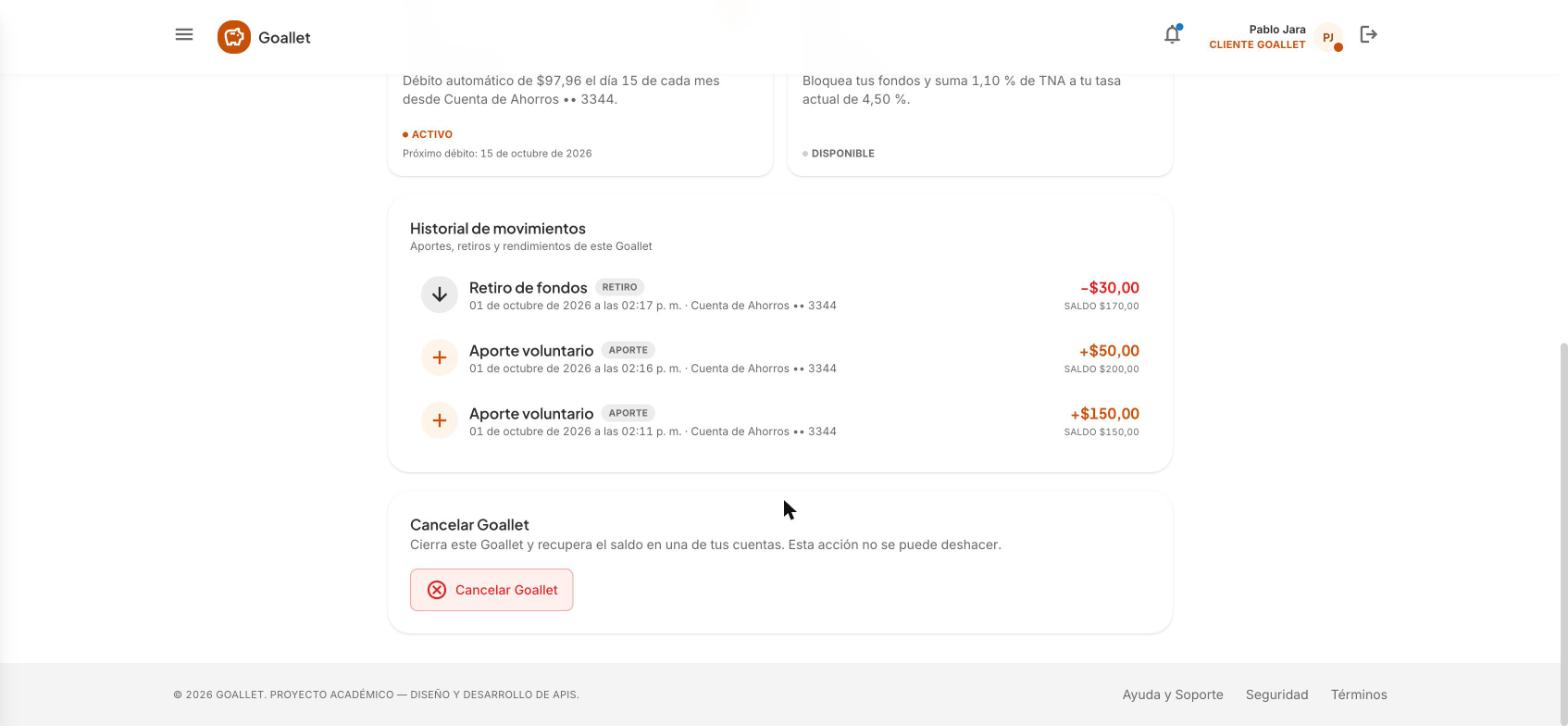
\includegraphics[width=0.9\linewidth]{../evidencias/fase-4-despliegue-frontend/14-historial-movimientos.jpg}
\caption{Historial de movimientos paginado por cursor}\label{fig:e2e-historial}
\end{figure}

\begin{figure}[H]
\centering
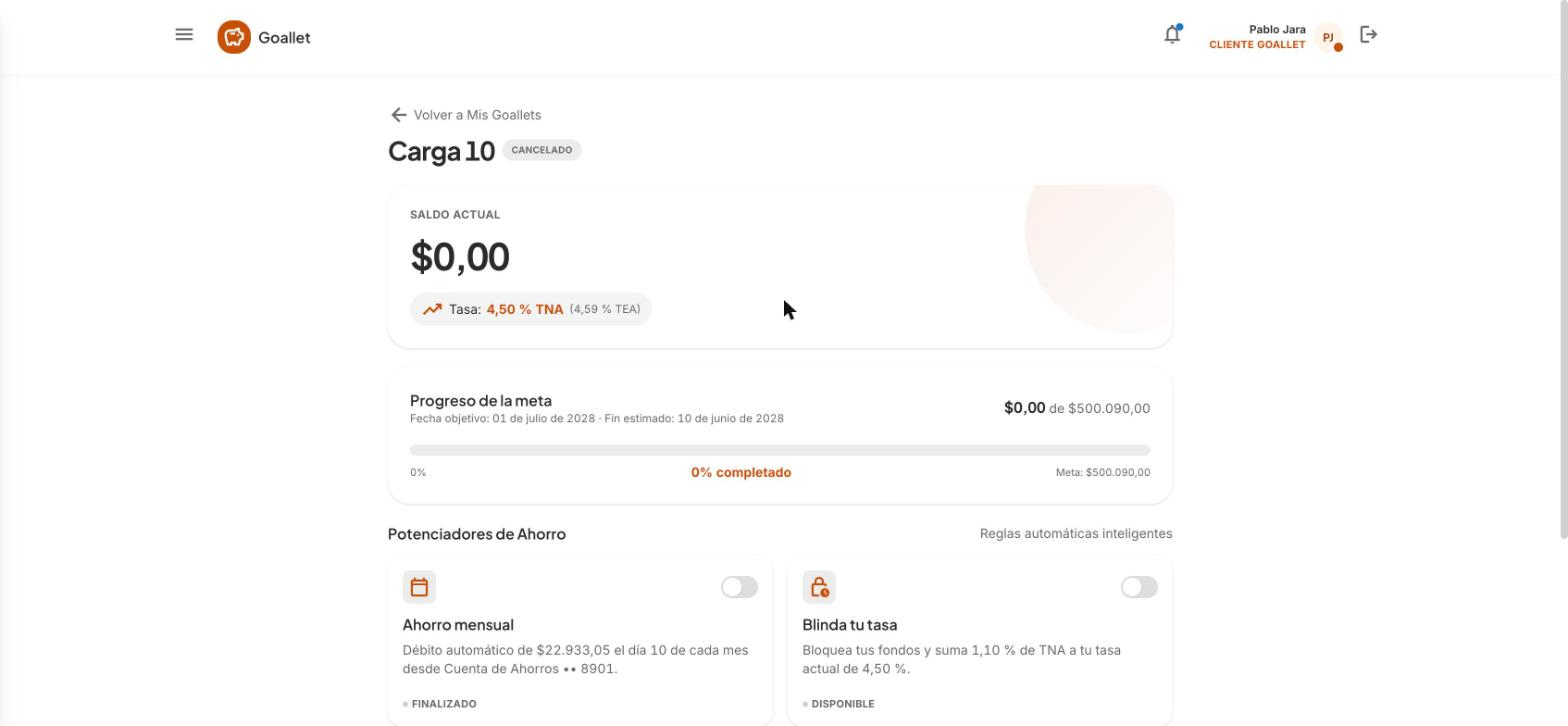
\includegraphics[width=0.9\linewidth]{../evidencias/fase-4-despliegue-frontend/17-plan-cancelado.jpg}
\caption{Plan cancelado}\label{fig:e2e-cancelado}
\end{figure}

Las 17 capturas del recorrido completo están en \texttt{docs/evidencias/fase-4-despliegue-frontend/}.

\chapter{Conclusiones y trabajo futuro}\label{cap:conclusiones}

\section{Conclusiones}

\begin{enumerate}
  \item \textbf{El enfoque API-First ordenó el trabajo del equipo.} Con el contrato OpenAPI como fuente de verdad, el frontend y el backend avanzaron en paralelo, y los cambios de alcance se discutieron sobre el contrato antes de escribir código.
  \item \textbf{Cada patrón responde a un requisito concreto.} El estilo híbrido REST y orientado a eventos resolvió el pico del corte diario y el desacoplamiento del Core; Adapter y Decorator aislaron el Core y su resiliencia; Strategy y State concentraron las reglas del negocio en código fácil de probar; el Transactional Outbox evitó perder eventos sin renunciar a la consistencia ACID del saldo.
  \item \textbf{La calidad se pudo medir.} Las 97 pruebas cubren el 97,9~\% de las líneas, y las pruebas de carga confirmaron los objetivos de la rúbrica: p95 de 336~ms y 0,001~\% de errores con 200 usuarios simultáneos, recuperación automática después de un pico de 500 usuarios y un punto de ruptura identificado en unas 220 peticiones por segundo.
  \item \textbf{Medir sacó a la luz problemas reales.} Las pruebas en el entorno desplegado revelaron una consulta al Core con dos viajes a la base, una caché de DNS del Gateway que provocaba errores 502 tras un redespliegue una configuración de TLS que aceptaba TLS~1.2 y, ya con el frontend integrado, una revalidación de caché HTTP (304) que mostraba saldos desactualizados. Los cuatro se corrigieron y se verificaron.
  \item \textbf{La automatización reduce el riesgo de cada cambio.} El pipeline ejecuta pruebas, valida el contrato, publica la imagen y despliega sin acceso SSH, con los secretos fuera del repositorio.
\end{enumerate}

\section{Trabajo futuro}

\begin{itemize}
  \item Mantener una tabla de saldos actualizada en la misma transacción que el ledger, para que las lecturas no recorran todos los movimientos, y migrar PostgreSQL a un servicio administrado.
  \item Escalar horizontalmente la API detrás del Gateway y separar la base de lecturas cuando el volumen lo justifique (CQRS).
  \item Incorporar un certificado TLS emitido por una autoridad reconocida y un dominio propio.
  \item Abrir el canal de socios (ahorro embebido) con una versión \texttt{v2} del contrato y credenciales propias por socio.
\end{itemize}


\printbibliography[heading=bibintoc,title={Referencias}]
\nocite{*}

\appendix
\chapter{Detalle de los patrones de diseño}\label{anx:patrones}
\input{generados/anexo-patrones}

\chapter{Evidencias}\label{anx:evidencias}

Todas las evidencias están en \texttt{docs/evidencias/} del repositorio. Se pueden regenerar con los scripts indicados en cada sección.

\section{Validación del contrato}
\lstinputlisting{../evidencias/fase-3-contrato/lint-redocly.txt}

\section{Pruebas unitarias y de integración}
\lstinputlisting{../evidencias/fase-4-pruebas/resumen-pruebas.txt}

\section{Seguridad contra la API desplegada}
Generadas con \texttt{docs/evidencias/generar-evidencias-api.sh}. Los tokens aparecen recortados.
\lstinputlisting{../evidencias/fase-4-seguridad/evidencias-seguridad.txt}

\section{Despliegue en AWS}
\lstinputlisting{../evidencias/fase-4-despliegue/recursos-aws.txt}
\lstinputlisting{../evidencias/fase-4-despliegue/servidor-contenedores.txt}

\section{Despliegue del frontend en Azure}
La suscripción y el tenant aparecen enmascarados.
\lstinputlisting{../evidencias/fase-4-despliegue-frontend/recursos-azure.txt}
\lstinputlisting{../evidencias/fase-4-despliegue-frontend/verificacion-frontend.txt}
\lstinputlisting{../evidencias/fase-4-despliegue-frontend/encender-apagar.txt}
\lstinputlisting{../evidencias/fase-4-despliegue-frontend/pipelines.txt}

\section{Pipeline de CI/CD}
\lstinputlisting{../evidencias/fase-4-despliegue/pipeline-ci-cd.txt}

\chapter{Distribución del trabajo}\label{anx:equipo}

La Tabla~\ref{tab:equipo} resume las responsabilidades principales de cada integrante según su aporte al repositorio. Todos los integrantes participaron en la revisión del diseño y se prepararon para defender cualquier parte del proyecto en la sustentación, como parte de la planificación del equipo.

\begin{table}[H]
\centering
\caption{Distribución del trabajo por integrante}\label{tab:equipo}
\begin{tabularx}{\linewidth}{@{}>{\raggedright}p{4.2cm} X@{}}
\toprule
\textbf{Integrante} & \textbf{Responsabilidades principales} \\
\midrule
Carlos Adrian Espinoza Alvarez & Alineación de la Fase~2 con el diseño, contrato OpenAPI~3.1, backend en Node.js por capas con sus patrones de diseño, seguridad (JWT RS256 y scopes), pruebas y cobertura, despliegue en AWS y Azure con CI/CD, pruebas de carga con k6, integración del frontend con la API e informe final. \\
Pablo Jara & Frontend en Next.js (ingreso, dashboard, Goallets, componentes y paleta de colores) y modelo ArchiMate bancario inicial. Administración del repositorio. \\
Miguel Lara & Visión de negocio y requerimientos (alcance), informe de la Fase~2, diagramas C4 en Structurizr, vista ArchiMate y servicio de autenticación JWT en la arquitectura. \\
Carina Torres & Core bancario simulado en MongoDB (modelo, poblado de datos, vistas y transacciones) y diagramas de contexto y de contenedores. \\
Sebastián Uyaguari & Documento de la Fase~1 y justificación del negocio, y análisis de los patrones de diseño. \\
\bottomrule
\end{tabularx}
\end{table}


\end{document}
